\documentclass{beamer}
\usepackage[utf8]{inputenc}
\usepackage[T1]{fontenc}
\usepackage[ngerman]{babel}
\usepackage{graphicx}
\usepackage{gensymb}
\usepackage{bold-extra}

\input{flat-blue-theme.inc}

\author{Hauke Stieler\\\href{mailto:4stieler@informatik.uni-hamburg.de}{4stieler@informatik.uni-hamburg.de}}
\title{OpenStreetMap}
\subtitle{What is that and how can I contribute?}
\date{\today}

\begin{document}
	\maketitle
	
	\begin{frame}
		\tableofcontents
	\end{frame}

	\section{What is this?}
	
	\begin{frame}
		\begin{itemize}
			\item free\footnote{\textit{free} as in \textit{free}dom} project collecting \textbf{free accessible} geodata
			\item open database for geodata
			\item ODC-ODbL
			\begin{itemize}
				\item OpenDataCommons Open Database License
				\item Ersetzt CC BY-SA 2.0 {\tiny (share alike \& attribution)}
			\end{itemize}
		\end{itemize}
	\end{frame}

	\subsection{Motivation}
	
	\begin{frame}
		Why has OpenStreetMap been created?
		\begin{itemize}
			\item proprietary maps old and faulty
			\item focus on cars and traffic
			\item no access to raw data
			\begin{itemize}
				\item error correction not possible
			\end{itemize}
			\item Google Maps \textit{not directly evil} -- but \textbf{not free}
			\item license problems with (nearly) all map service providers
		\end{itemize}
	\end{frame}

	\subsection{History}

	\begin{frame}
		\begin{itemize}
			\item 2004 -- OSM founded
			\item 2006 -- release JOSM-Editor
			\item 2006 -- first map rendered with Mapnik
			\item 2007 -- TIGER data import USA started
			\item 2008 -- TIGER data import USA finished
			\item 2009 -- API 0.6 (still latest version)
			\item 2009 -- cooperation with Wikipedia
			\item 2010 -- Bing Imagery allowed usage for OSM
			\item 2013 -- 1 mio. registered users
			\item 2016 -- Maps.me app enabled edits
		\end{itemize}
	\end{frame}

	\subsection{Statistics}

	\begin{frame}
		\begin{center}
			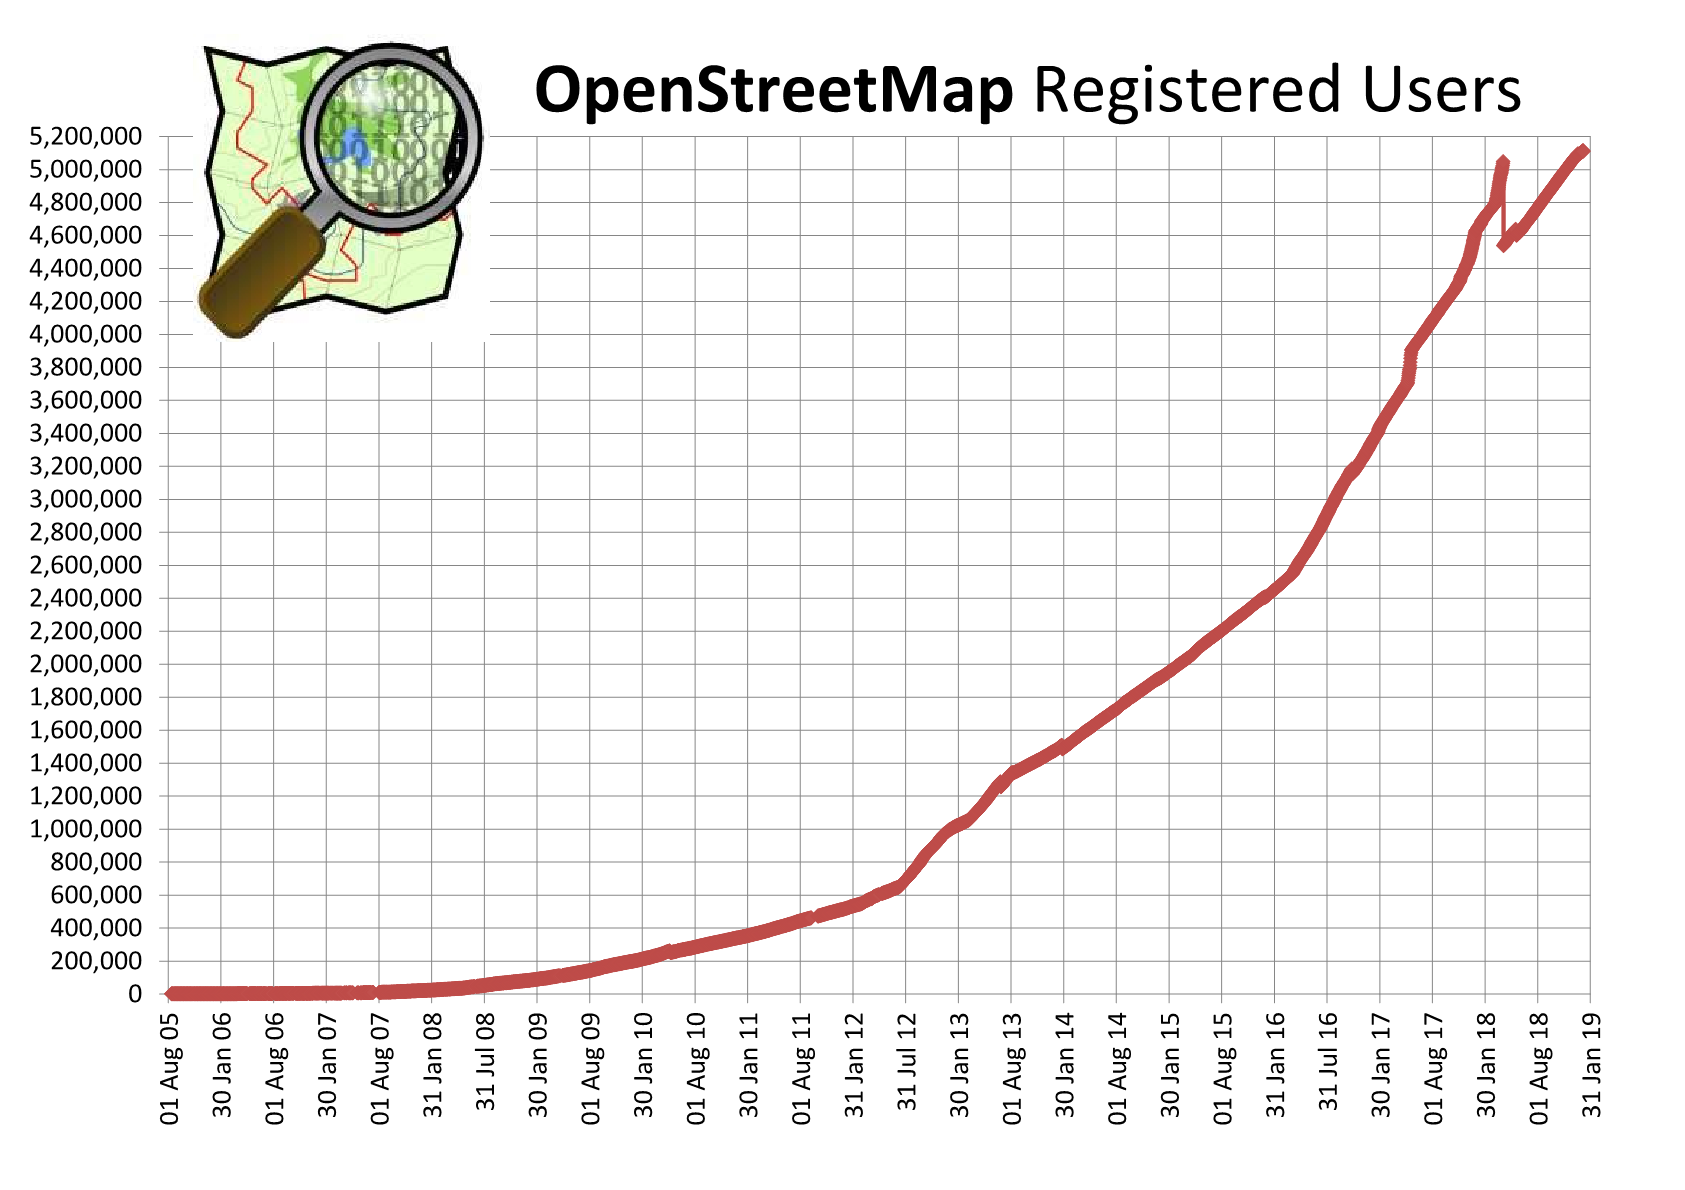
\includegraphics[width=\textwidth,height=\textheight,keepaspectratio]{images/Osmdbstats1_users.png}
		\end{center}
	\end{frame}

	\begin{frame}
		\begin{center}
			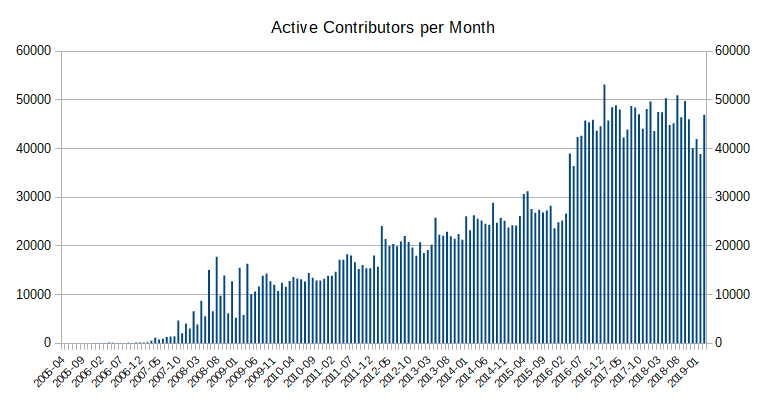
\includegraphics[width=\textwidth,height=\textheight,keepaspectratio]{images/Active_contributors_month.png}
		\end{center}
	\end{frame}
	
	\begin{frame}
		\begin{center}
			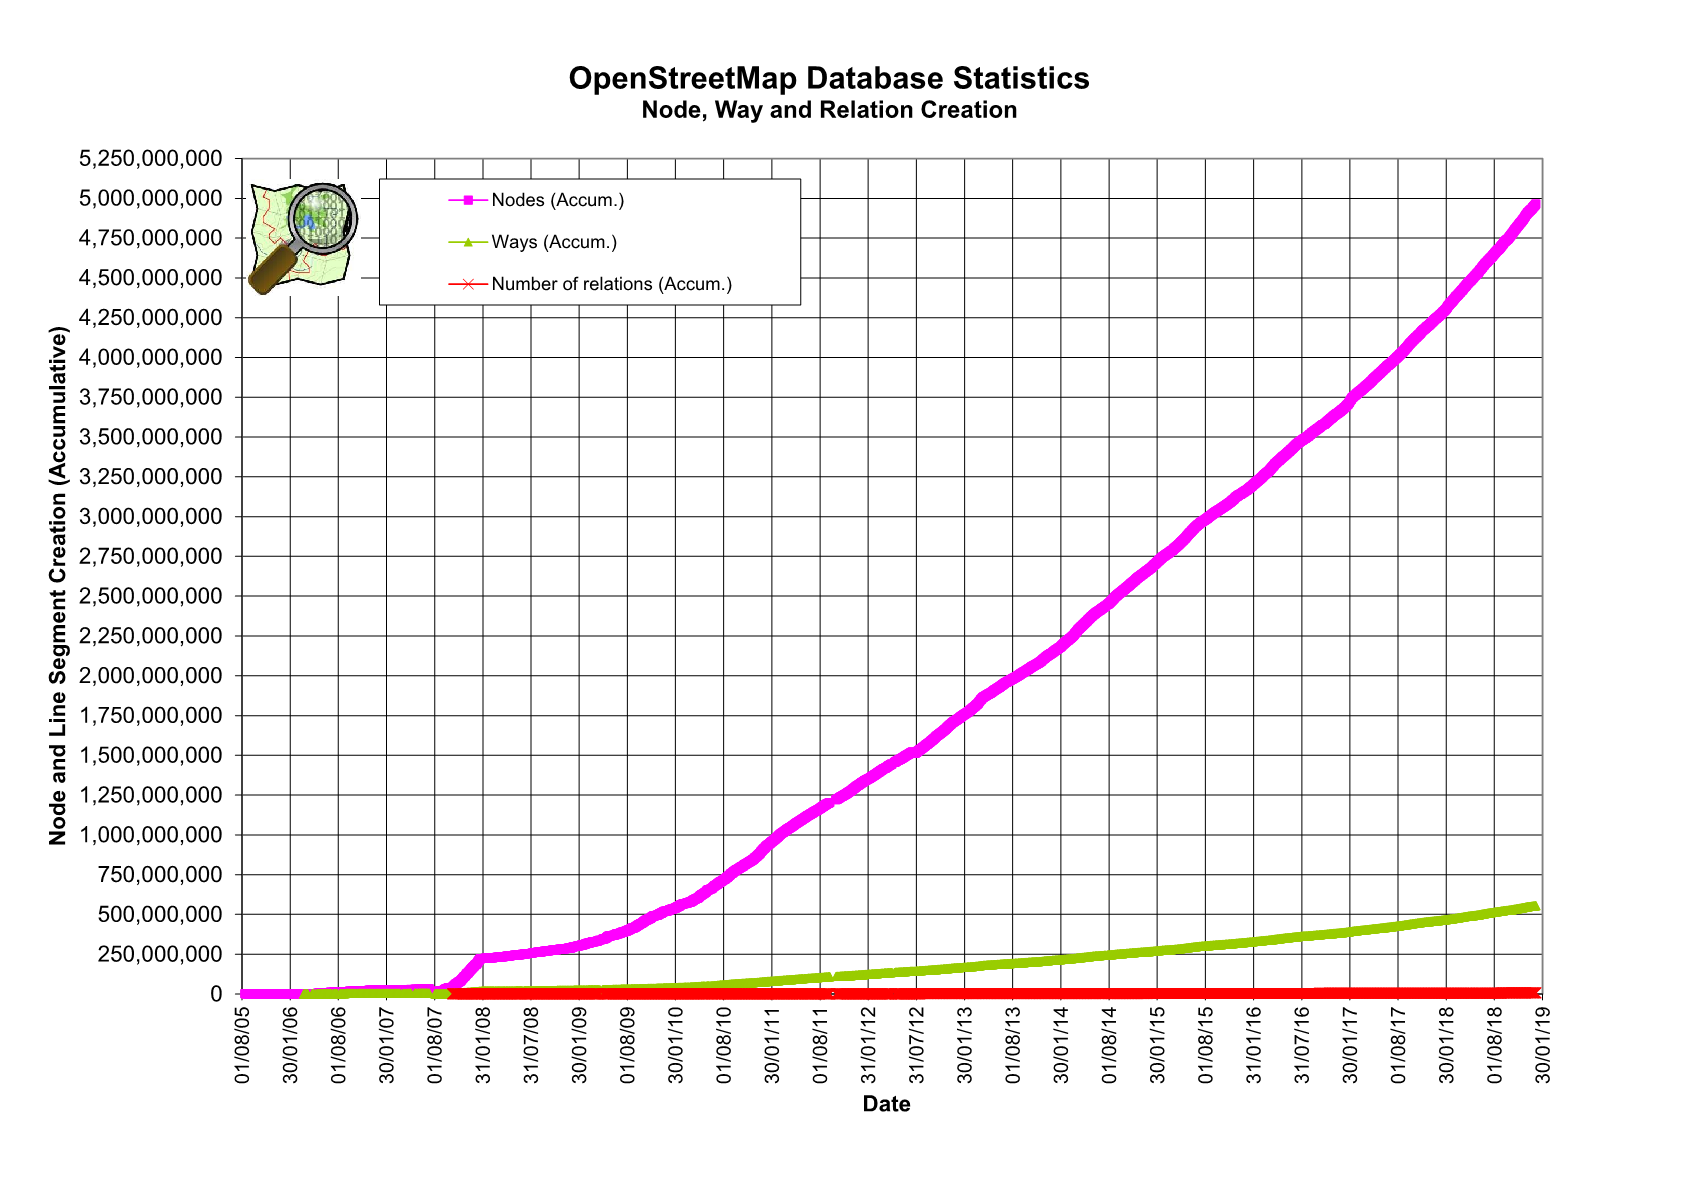
\includegraphics[width=\textwidth,height=\textheight,keepaspectratio]{images/Osmdbstats2.png}
		\end{center}
	\end{frame}
	
	\begin{frame}
		\begin{center}
			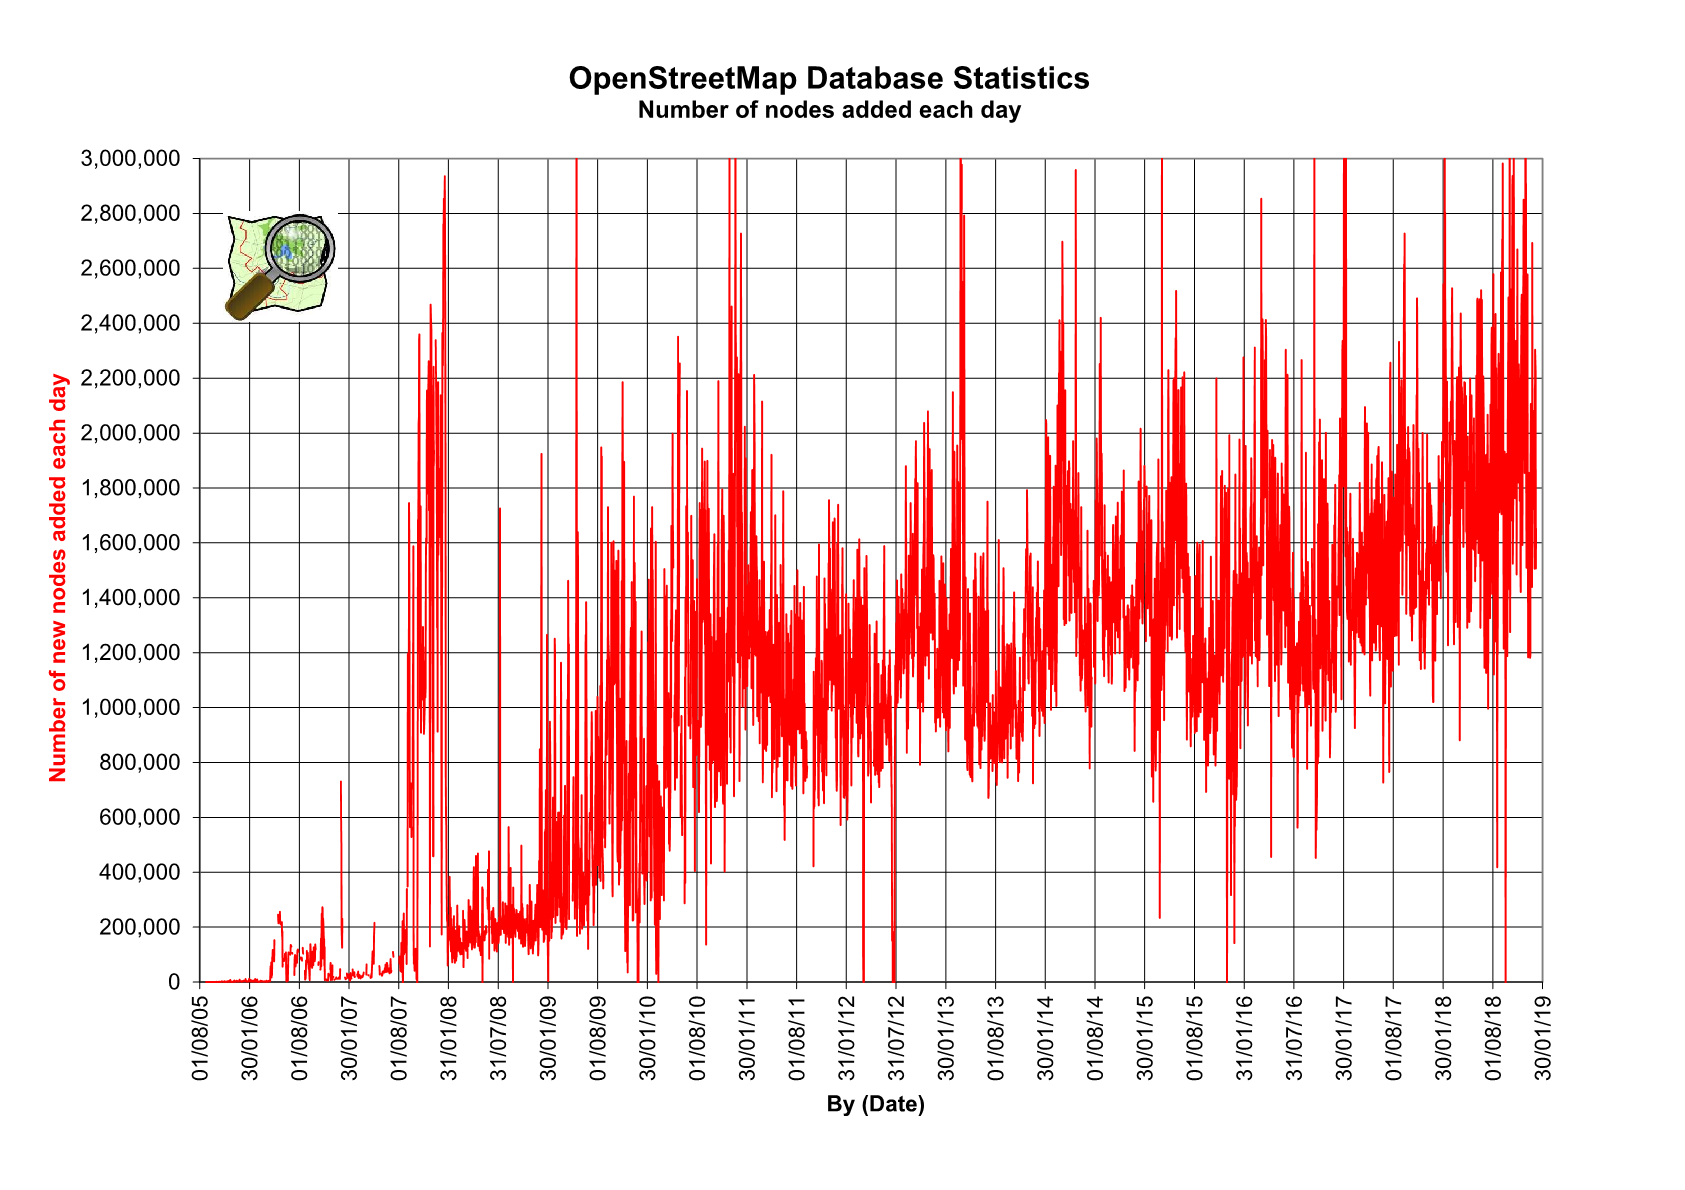
\includegraphics[width=\textwidth,height=\textheight,keepaspectratio]{images/Osmdbstats7A.png}
		\end{center}
	\end{frame}
	
	\begin{frame}
		\begin{center}
			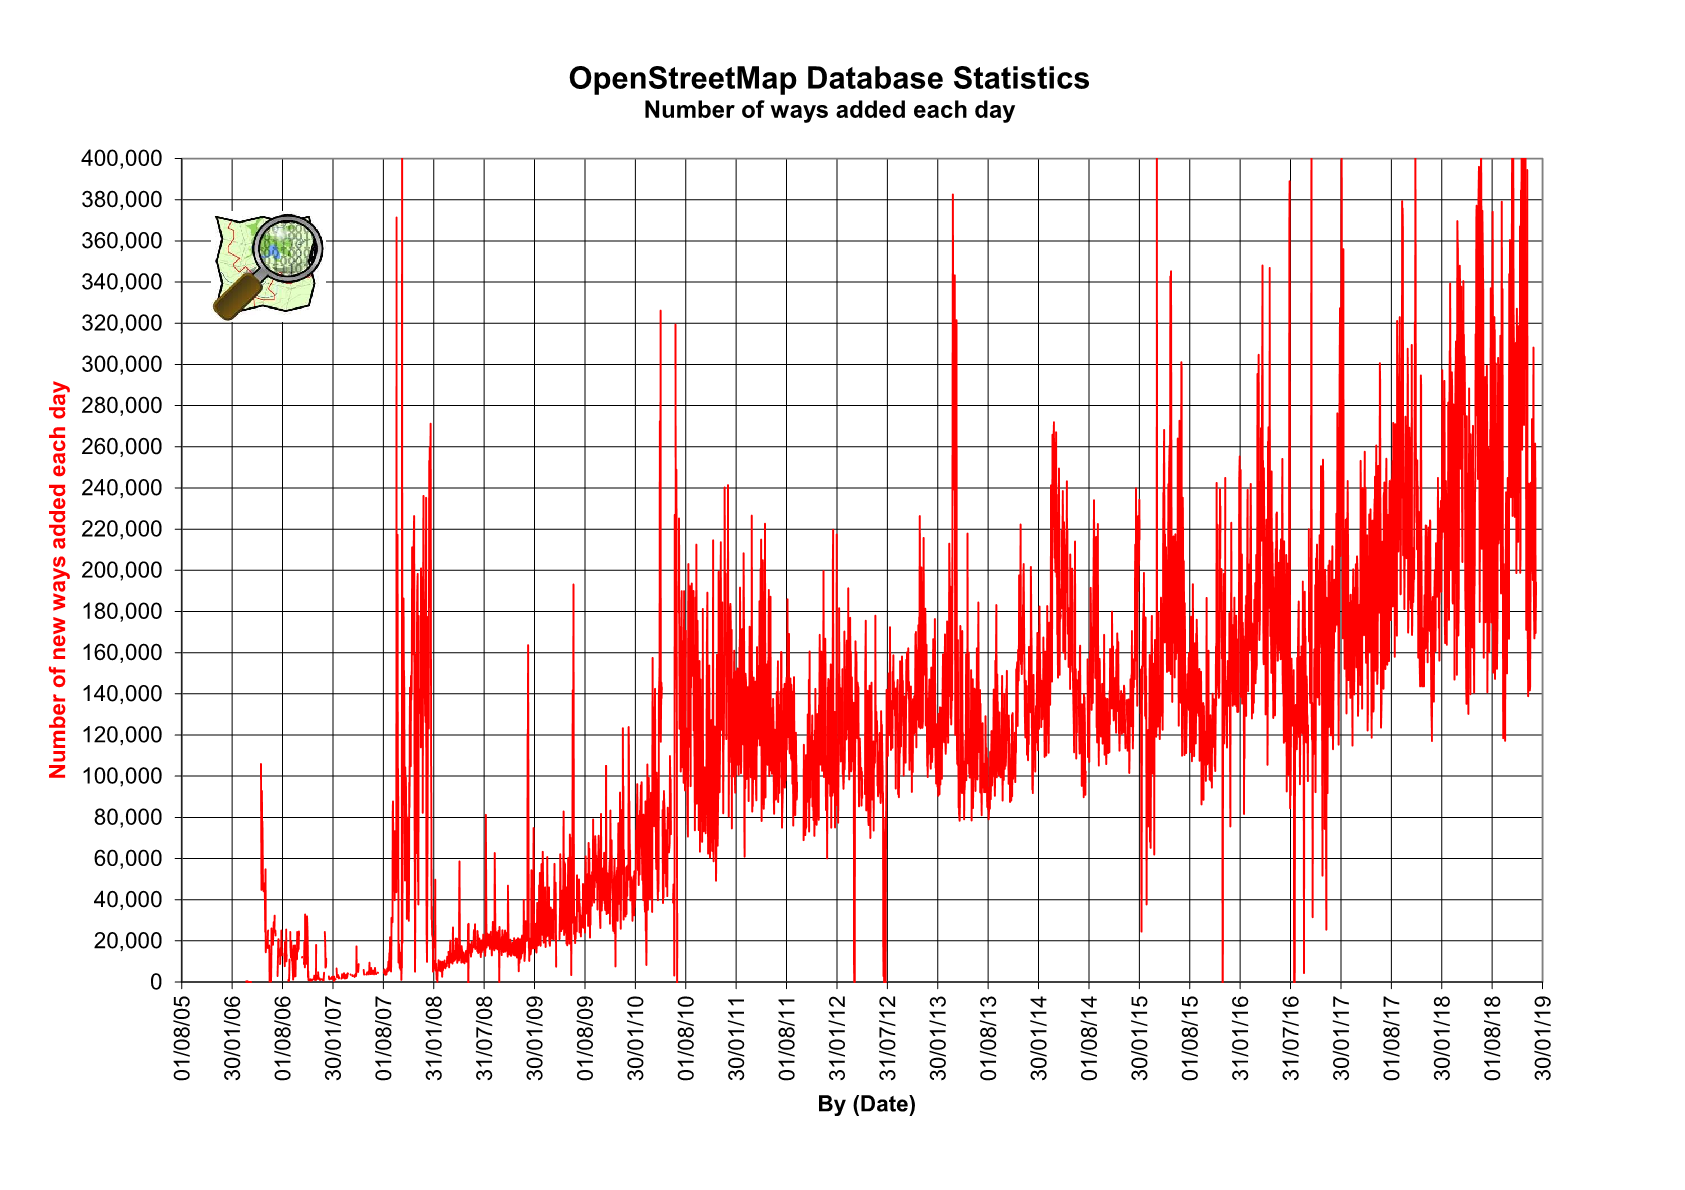
\includegraphics[width=\textwidth,height=\textheight,keepaspectratio]{images/Osmdbstats7B.png}
		\end{center}
	\end{frame}

	\subsection{Community}

	\begin{frame}{What is done?}
		\begin{itemize}
			\item developing software and tools
			\item actual mapping
			\item creating and maintaining documentation
			\item doing public relations activities
		\end{itemize}
	\end{frame}

	\begin{frame}{How is it done?}
		\begin{itemize}
		\item going outside collecting information
		\item using imagery services
		\item meet other mappers
		\item participating in a mapathon
		\end{itemize}
	\end{frame}
\end{document}












